\header{5}
\chapter{Reglementen \& Voorrangsregels}
\section{Inleiding}
In dit hoofdstuk gaan we kijken naar de regels en wetten op het water. Op de meeste wateren waar jullie zullen varen wordt gebruik gemaakt van het Binnenvaart Politie Reglement, het BPR. Het BPR bevat alle regels over hoe je met elkaar om moet gaan op het water.

\section{Algemene reglementen}
Om het BPR goed te kunnen begrijpen, zullen we eerst een aantal algemene zaken bespreken. We beginnen met vier definities; motorschip, zeilschip, klein schip en groot schip. 

\begin{itemize}
    \item \textbf{Motorschip:} Een schip dat mechanische middelen gebruikt om zich voort te bewegen, een motor dus.
    \item \textbf{Zeilschip:} Een schip dat \textbf{alleen} zijn zeilen gebruikt om voort te bewegen. Hier onder valt ook een surfplank, maar niet een zeilboot met een motor aan.
    \item \textbf{Klein schip:} Alle schepen onder de 20 meter, met uitzondering van: passagiersschip \footnote{Draagt overdag een gele ruit achter op het schip om dit aan te duiden}, veerpont, visser, sleepboot
(alleen als deze grote schepen sleept), duwboot en duwbak. Deze uitzonderingen zijn altijd grote schepen. 
    \item \textbf{Groot schip:} Schepen groter dan 20 meter, inclusief de eerdergenoemde uitzonderingen 
\end{itemize}

\subsection{Goed zeemanschap}
Het goed zeemanschap is een hele belangrijke regel op het water. Deze regel houdt in dat de schipper bij het ontbreken van duidelijke regels \textbf{alle nodige voorzorgsmaatregelen} moet nemen om de veiligheid te garanderen, schade te voorkomen of de doorstroom op het water te versoepelen. Ook mag een schipper voor eigen veiligheid of die van anderen afwijken van het BPR.

\subsection{Andere reglementen}
Het BPR geldt niet op alle wateren. Het is verstandig om vooraf (als je op voor jou onbekende wateren gaat varen) uit te zoeken welke regels er gelden. Dit kan bijvoorbeeld in de ANWB Wateralmanak. In deel 1 staan alle regels en wetten die gelden in Nederland en België. 

\newpage
\section{Voorrangsregels}
Voorrangssituaties zijn te verdelen in drie types: kruisende koersen, tegengestelde koeren en oplopende koersen. Deze drie zijn te zien in figuur \ref{pic:voorrangkoers}. Welke van deze situaties je vaart bepaalt met welke regels je te maken hebt. 
\begin{figure}[H]
    \centering
    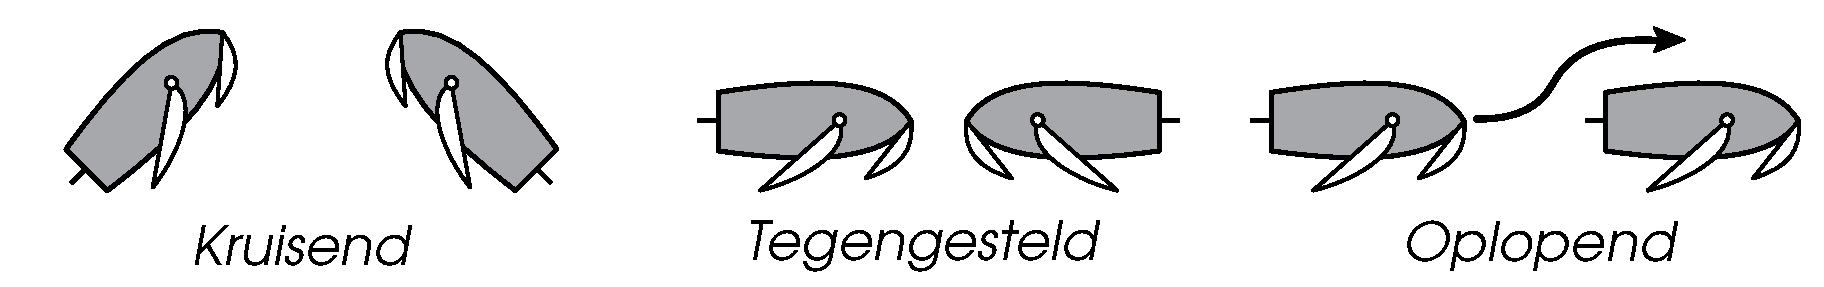
\includegraphics[width=0.8\textwidth]{Hoofdstukken/Reglementen/pdf/voorrangskoersen.pdf}
    \caption{Voorrangskoersen}
    \centering
    \label{pic:voorrangkoers}
\end{figure}
De voorrangsregels hebben ook een volgorde. Na het bepalen van welke koers je vaart, kijk je altijd eerst naar de bovenste regel die hierbij hoort. Als deze regel niet van toepassing is, ga je pas door naar de volgende. Dit doe je net zo lang tot er een regel is die toe te passen is op jouw situatie.


\paragraph{Kruisende koersen}
\vspace{-0.7cm}
\begin{figure}[H]
	\centering
	\begin{minipage}[t]{0.70\textwidth}
		\textbf{1.} Het schip wat aan de stuurboordswal vaart heeft voorrang.\\
		\textit{Zeilschip A vaart aan de stuurboordswal en heeft voorrang op B}
	\end{minipage}
	\hfill
	\begin{minipage}[t]{0.20\textwidth}
		\raisebox{-0.5\height}{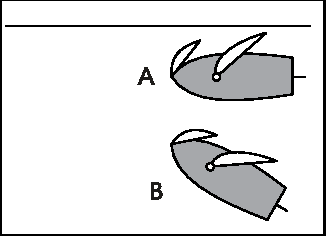
\includegraphics[width=\textwidth]{Hoofdstukken/Reglementen/pdf/kruis_stuurboordswal.pdf}}
		\label{pic:kr1}
	\end{minipage}
	\hfill
\end{figure}

\vspace{-0.7cm}

\begin{figure}[H]
	\centering
	\begin{minipage}[t]{0.70\textwidth}
		\textbf{2.} Grote schepen hebben voorrang op kleine schepen.\\
		\textit{Het grote motorschip A heeft voorrang op het kleine motorschip B}
	\end{minipage}
	\hfill
	\begin{minipage}[t]{0.20\textwidth}
		\raisebox{-0.5\height}{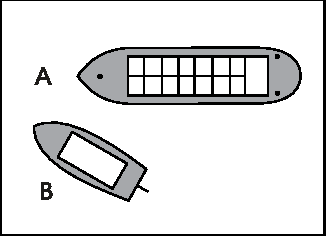
\includegraphics[width=\textwidth]{Hoofdstukken/Reglementen/pdf/kruis_groot_klein.pdf}}	
		\label{pic:kr2}
	\end{minipage}
	\hfill
\end{figure}

\vspace{-0.7cm}
\begin{figure}[H]
	\centering
	\begin{minipage}[t]{0.72\textwidth}
		\textbf{3.} Schepen op het hoofdvaarwater gaan voor op het nevenvaarwater.\\
		\textit{Motorschip A op het hoofddvaarwater heeft voorrang op motorschip B}
	\end{minipage}
	\hfill
	\begin{minipage}[t]{0.20\textwidth}
		\raisebox{-0.5\height}{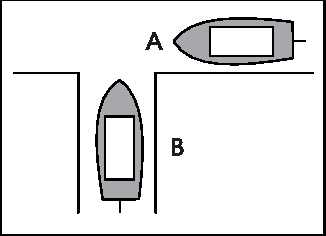
\includegraphics[width=\textwidth]{Hoofdstukken/Reglementen/pdf/kruis_hoofd_neven.pdf}}	
		\label{pic:kr3}
	\end{minipage}
	\hfill
\end{figure}

\vspace{-0.7cm}
\begin{figure}[H]
	\centering
	\begin{minipage}[t]{0.70\textwidth}
		\textbf{4.} Een zeilschip gaat voor een roeiboot gaat voor een motorschip.\\
		\textit{Zeilschip A heeft voorrang op roeiboot B en motorschip C\\
			Roeiboot B heeft voorrang op motorschip C}
	\end{minipage}
	\hfill
	\begin{minipage}[t]{0.20\textwidth}
		\raisebox{-0.65\height}{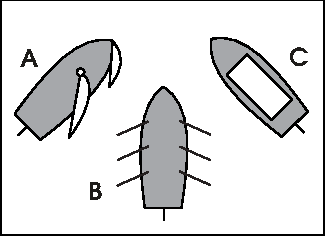
\includegraphics[width=\textwidth]{Hoofdstukken/Reglementen/pdf/kruis_zsm.pdf}}	
		\label{pic:kr4}
	\end{minipage}
	\hfill
\end{figure}

\vspace{-0.7cm}
\begin{figure}[H]
	\centering
	\begin{minipage}[t]{0.70\textwidth}
		\textbf{5.} Motor- en roeiboten onderling: Het schip van rechts gaat voor.\\
		\textit{Motorschip A op rechts heeft voorrang op motorschip B}
	\end{minipage}
	\hfill
	\begin{minipage}[t]{0.20\textwidth}
		\raisebox{-0.65\height}{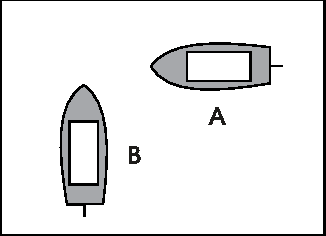
\includegraphics[width=\textwidth]{Hoofdstukken/Reglementen/pdf/kruis_motor_onderling.pdf}}	
		\label{pic:kr5}
	\end{minipage}
	\hfill
\end{figure}

\vspace{-0.7cm}

\textbf{6.} Bij zeilschepen onderling zijn de volgende twee regels van belang:
\vspace{-0.5cm}
\begin{figure}[H]
	\centering
	\hspace{0.02\textwidth}
	\begin{minipage}[t]{0.70\textwidth}
		\textbf{6.1}. Een zeilschip met zeilen over bakboord heeft voorrang.\\
		\textit{Zeilschip B (met zijn zeilen over bakboord) heeft voorrang op \\zeilschip A (met zijn zeilen over stuurboord)}
	\end{minipage}
	\hfill
	\begin{minipage}[t]{0.20\textwidth}
		\raisebox{-0.6\height}{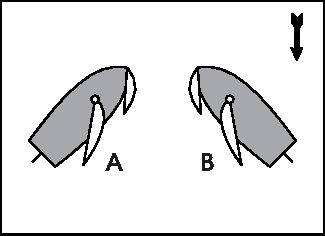
\includegraphics[width=\textwidth]{Hoofdstukken/Reglementen/pdf/kruis_zeilboot_onderling_bakboord.pdf}}	
		\label{pic:kr41}
	\end{minipage}
	\hfill
\end{figure}

\vspace{-0.7cm}
\begin{figure}[H]
	\centering
	\hspace{0.02\textwidth}
	\begin{minipage}[t]{0.70\textwidth}
		\textbf{6.2.} Een zeilschip aan loef wijkt voor een zeilschip aan lij.\\
		\textit{Zeilschip A ligt aan loef van zeilschip B en verleent dus voorrang}
	\end{minipage}
	\hfill
	\begin{minipage}[t]{0.20\textwidth}
		\raisebox{-0.55\height}{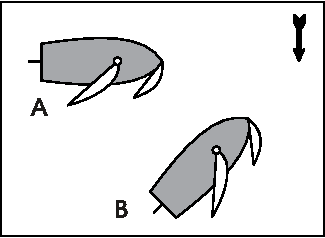
\includegraphics[width=\textwidth]{Hoofdstukken/Reglementen/pdf/kruis_zeilboot_onderling_loef_lij.pdf}}	
		\label{pic:kr42}
	\end{minipage}
	\hfill
\end{figure}

\paragraph{Tegengestelde koersen}
\vspace{-0.2cm}
\begin{figure}[H]
	\centering
	\begin{minipage}[t]{0.70\textwidth}
		\textbf{1.} Het schip wat aan de stuurboordswal vaart heeft voorrang.\\
		\textit{Zeilschip B vaart aan de stuurboordswal en heeft voorrang op A}
	\end{minipage}
	\hfill
	\begin{minipage}[t]{0.25\textwidth}
		\raisebox{-0.55\height}{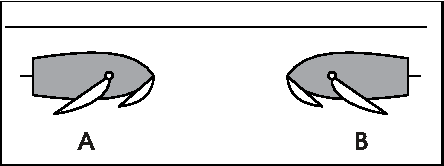
\includegraphics[width=\textwidth]{Hoofdstukken/Reglementen/pdf/tegen_stuurboord.pdf}}
		\label{pic:tg1}
	\end{minipage}
	\hfill
\end{figure}
\vspace{-0.7cm}

\begin{figure}[H]
	\centering
	\begin{minipage}[t]{0.70\textwidth}
		\textbf{2.} Grote schepen hebben voorrang op kleine schepen.\\
		\textit{Het grote motorschip B heeft voorrang op het kleine motorschip A}
	\end{minipage}
	\hfill
	\begin{minipage}[t]{0.25\textwidth}
		\raisebox{-0.55\height}{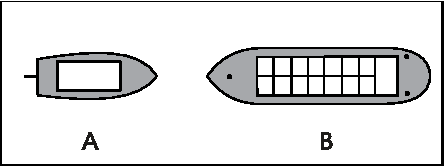
\includegraphics[width=\textwidth]{Hoofdstukken/Reglementen/pdf/tegen_groot_klein.pdf}}
		\label{pic:tg2}
	\end{minipage}
	\hfill
\end{figure}
\vspace{-0.7cm}

\begin{figure}[H]
	\centering
	\begin{minipage}[t]{0.70\textwidth}
		\textbf{3.} Een zeilschip gaat voor een roeiboot gaat voor een motorschip.\\
		\textit{Zeilschip A heeft voorrang op roeiboot B \\
			Zeilschip C heeft voorrang op motorschip D \\
			Roeiboot E heeft voorrang op motorschip F}
	\end{minipage}
	\hfill
	\begin{minipage}[t]{0.25\textwidth}
		\raisebox{-0.75\height}{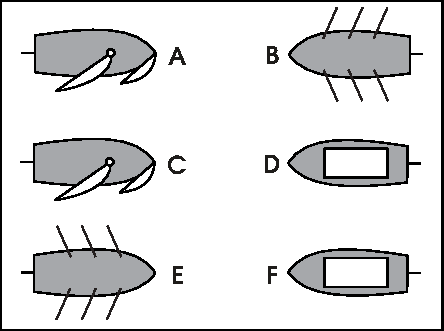
\includegraphics[width=\textwidth]{Hoofdstukken/Reglementen/pdf/tegen_zsm.pdf}}
		\label{pic:tg3a}
	\end{minipage}
	\hfill
\end{figure}
\vspace{-0.7cm}

\begin{figure}[H]
	\centering
	\begin{minipage}[t]{0.70\textwidth}
		\textbf{4.} Zeilschepen onderling: Een zeilschip met zeilen over bakboord heeft voorrang.\\
		\textit{Zeilschip B (met zijn zeilen over bakboord) heeft voorrang op A}
	\end{minipage}
	\hfill
	\begin{minipage}[t]{0.25\textwidth}
		\raisebox{-0.75\height}{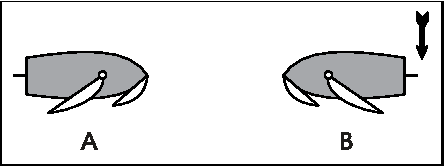
\includegraphics[width=\textwidth]{Hoofdstukken/Reglementen/pdf/tegen_zeilboot_onderling.pdf}}	
		\label{pic:tg4}
	\end{minipage}
	\hfill
\end{figure}
\vspace{-0.7cm}

\begin{figure}[H]
	\centering
	\begin{minipage}[t]{0.70\textwidth}
		\textbf{5.} Roei- of motorschepen onderling: Beide wijken naar stuurboord.\\
		\textit{Beide motorschepen wijken naar stuurboord}
	\end{minipage}
	\hfill
	\begin{minipage}[t]{0.25\textwidth}
		\raisebox{-0.55\height}{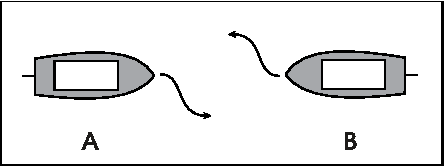
\includegraphics[width=\textwidth]{Hoofdstukken/Reglementen/pdf/tegen_motor_spier_onderling.pdf}}	
		\label{pic:tg5}
	\end{minipage}
	\hfill
\end{figure}

\paragraph{Oplopen}
Oplopen is \textit{enkel} toegestaan wanneer dit gedaan kan worden zonder gevaar voor andere schepen. Oplopen wordt voornamelijk langs bakboord gedaan. Het is echter ook toegestaan, wanneer de situatie hier om vraagt, om langs stuurboord op te lopen.

\begin{figure}[H]
	\centering
	\begin{minipage}[t]{0.70\textwidth}
		Zeilschepen onderling lopen elkaar op via de loefzijde. Hierdoor neem je de wind uit de zeilen van het opgelopen schip en gaat het oplopen sneller. Tijdens het oplopen mag medewerking verlangd worden van het opgelopen schip.
	\end{minipage}
	\hfill
	\begin{minipage}[t]{0.25\textwidth}
		\raisebox{-0.8\height}{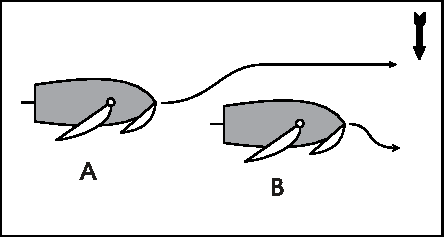
\includegraphics[width=\textwidth]{Hoofdstukken/Reglementen/pdf/oplopen.pdf}}
		\label{pic:op}
	\end{minipage}
	\hfill
\end{figure}

\newpage
\subsection{Voorrangsregels op een rij}
Om de voorrangsregels makkelijk te kunnen onthouden staan ze hieronder samengevat:\\[0.1cm]
Bij \textbf{kruisende koersen} kijk je naar de volgende regels:
\vspace*{-0.15cm}
\begin{enumerate}
	\item Het stuurboordswal varende schip gaat voor
	\item Grote schepen gaan voor op kleine schepen
	\item Hoofdwater gaat voor nevenwater
	\item Zeilschip gaat voor roeiboot gaat voor motorschip
	\item Roei- of motorschepen onderling: het schip van rechts gaat voor
	\item Zeilschepen onderling: 
	\stepcounter{enumi}
	\begin{enumerate}
		\item [1.]Zeilen over bakboord gaat voor
		\item [2.]Loef wijkt voor lij
	\end{enumerate}
\end{enumerate}

Bij \textbf{tegengestelde koersen} kijk je naar de volgende regels:
\vspace*{-0.15cm}
\begin{enumerate}
	\item Het stuurboordswal varende schip gaat voor
	\item Grote schepen gaan voor op kleine schepen
	\item Zeilschip gaat voor roeiboot gaat voor motorschip
	\item Zeilschepen onderling: zeilen over bakboord gaat voor
	\item Roei- of motorschepen onderling: beiden wijken naar stuurboord
\end{enumerate}

Bij \textbf{oplopende koersen}, wijkt de oploper uit. Het opgelopen schip kan indien nodig uitwijken.

\subsection{Toevoegingen}
\begin{figure}[H]
	\centering
	\begin{minipage}[t]{0.65\textwidth}
		Wanneer je vaarwater oversteekt, heb je geen voorrang. Andere schepen moeten hun koers en snelheid niet of nauwelijks hoeven aan te passen voor jouw manoeuvre. \\
		
		
		De regel `Stuurboordswal gaat voor' gaat over de stuurboordszijde van het \textbf{vaarwater}, niet over de echte wal. Boot A en B in figuur \ref{pic:SBwal} varen dus beide aan stuurboordswal, ondanks dat zij niet aan een fysieke wal varen.
	\end{minipage}
	\hfill
	\begin{minipage}[t]{0.30\textwidth}
		\raisebox{-0.9\height}{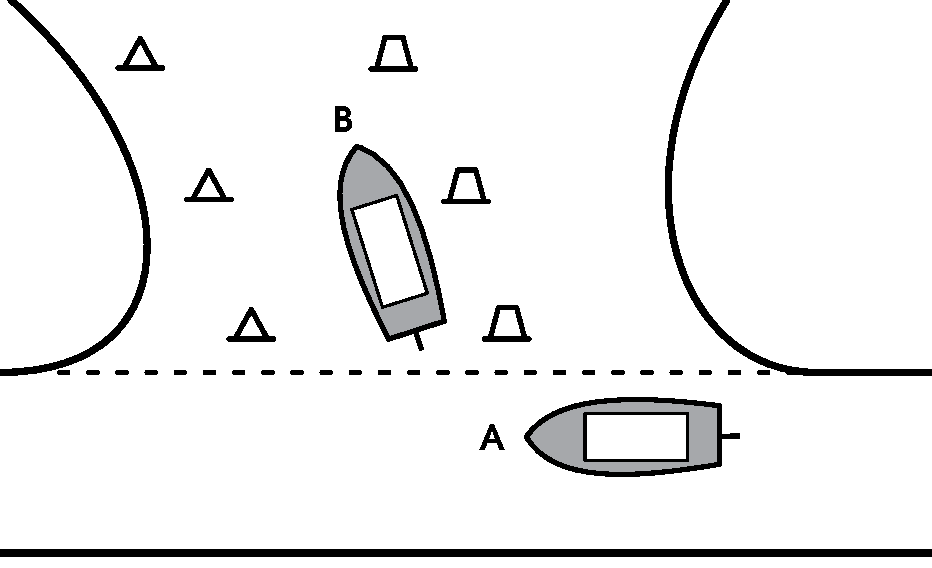
\includegraphics[width=\textwidth]{Hoofdstukken/Reglementen/pdf/sb_wal.pdf}}
		\caption{}
		\label{pic:SBwal}
	\end{minipage}
\end{figure}


\section{Conclusie}
Na het lezen van dit hoofdstuk heb je verstand van de voorrangsregels op het water. Een van de belangrijkste is het goed zeemanschap, wat inhoudt dat je alles doet om een gevaarlijke situatie of aanvaring te voorkomen. Daarnaast ken je de verschillende voorrangssituaties en volgorde en weet je hoe je de regels moet toepassen. 